\chapter{Architettura}

In questo capitolo verranno descritte le scelte architetturali e implementative che stanno alla base del contributo di questa tesi al progetto IoE. 

Lo scenario legato alla mobilità elettrica veicolare è caratterizzato dalla presenza di diversi domini applicativi, piattaforme e parti interessate i quali necessitano di comunicare in modo unificato e trasparente. A tal fine è stato utilizzato il progetto Smart-M3 (\cite{tullio2011}), cuore della nostra architettura. Appoggiandosi sulle tecnologie tipiche del \emph{Semantic Web}, Smart-M3 assicura l'interoperabilità tra gli attori in gioco. 

In particolare vedremo come possono coesistere elementi reali ed elementi simulati e come il passaggio dall'uno all'altro sia assolutamente trasparente a tutti i componenti del sistema grazie all'uso di tecnologie ontology-based.

\section{Smart-M3}\label{sec:smart-m3}

Prima di parlare dei componenti strettamente legati a questo progetto è doveroso fare un introduzione alla tecnologia che fa da collante tra di essi, ovvero Smart-M3. Capire come funziona Smart-M3 e quali sono i suoi principi è fondamentale per comprendere a fondo il seguito di questo documento.

M3 è un architettura middleware che realizza l'interoperabilità delle informazioni in maniera cross-domain, multi-vendor, multi-device, multi-piattaforma (\cite{smart2013}). Smart-M3 è la sua prima implementazione Open Source, proposta da SOFIA, un Progetto Europeo (2009-11) appartenente al framework ARTEMIS. 
La piattaforma implementa il disaccoppiamento tra produttori e consumatori di informazione. In questa architettura tutti gli attori (sensori, dispositivi, servizi, attuatori ecc..) cooperano attraverso un database RDF che è lo standard deciso dal World Wide Web Consortium per la descrizione di informazioni e concetti. L'interoperabilità è resa possibile da un modello di dati condiviso che si basa su tecnologie tipiche del Semantic Web.

Il Semantic Web è un framework sviluppato dal World Wide Web Consortium per consentire la condivisione e il riutilizzo dei dati attraverso  applicazioni, aziende e comunità eterogenee.

La figura ~\ref{fig:smart-m3} mostra il funzionamento dell'architettura M3. Il ``legacy gate'' è un interfaccia con il mondo esterno e possono coesisterne molteplici istanze in un architettura M3.

\begin{figure}[H]
	\centering
	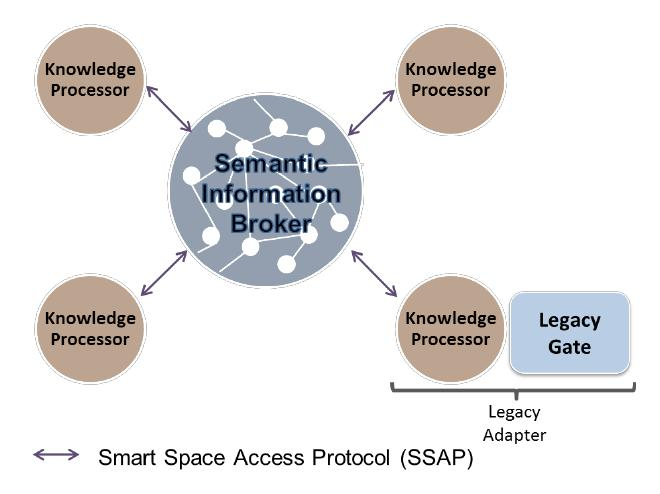
\includegraphics[width=0.5\textwidth]{assets/smart-m3.jpg}
	\caption{Architettura Smart-M3}
	\label{fig:smart-m3}
\end{figure}

\subsection{Semantic Information Broker}\label{subsec:sib}

Il \emph{Semantic Information Broker} (SIB) è l'entità responsabile della conservazione e della gestione delle informazioni condivise nell'architettura M3. Gli agenti Software che si scambiano le informazioni vengono chiamati \emph{Knowledge Processors} (KP). L'accesso alla SIB da parte dei KP avviene attraverso lo \emph{Smart Space Access Protocol}  (SSAP) basato su messaggi XML scambiati attraverso socket TCP/IP. Vengono fornite API che implementano il protocollo SSAP in diversi linguaggi.

Il SIB è un architettura a 5 livelli (\cite{smart2010}) come mostrato in figura ~\ref{fig:sib-architecture}:

\begin{enumerate}
	\item \textbf{Transport}: Gestisce una o più comunicazioni di rete a livello di trasporto, permettendo al SIB di comunicare con diverse reti e architetture. Il livello di trasporto è collegato a quello sottostante tramite il DBus, rendendo possibile l'aggiunta e la rimozione di connettori a runtime.
	\item \label{enum:handling}\textbf{Operation Handling}: Gestisce le diverse operazioni del protocollo SSAP ognuna delle quali viene eseguita in un thread dedicato. Malgrado l'uso intensivo di thread possa degradare le performance,  è stata ritenuta determinante la chiarezza di codice che ne consegue.
	\item \label{enum:graph}\textbf{Graph Operations}: Gestisce le operazioni di inserimento, rimozione e query dal database RDF come richiesto dal livello ~\ref{enum:handling}. Viene eseguito all'interno di un singolo thread che schedula ed esegue le richieste provenienti dai thread che gestiscono le operazioni SSAP la cui comunicazione avviene tramite code asincrone.
	\item \textbf{Triple Operations}: Gestisce le operazioni SPARQL, WQL e le query basate su pattern-matching di triple RDF. Attualmente è implementato tramite Piglet, un database RDF che si appoggia ad SQL lite per la persistenza delle informazioni. Lo strato può essere tranquillamente cambiato a patto che si scriva il codice necessario ad interfacciare le operazioni a livello di grafo (~\ref{enum:graph}) con l'interfaccia fornita dal nuovo store RDF.
	\item \textbf{Persistent storage}: Assicura la persistenza dei dati.
\end{enumerate}

\subsection{I Knowledge Processor}

I Knowledge Processor (KP) sono le parti attive dell'architettura Smart-M3. Un KP interagisce con il SIB non direttamente tramite il protocollo SSAP ma tramite le Knowledge Processor Interface (KPI) ovvero le librerie che lo implementano. Queste possono trovarsi a qualunque livello di astrazione ed essere scritte in qualunque linguaggio. Le funzioni messe a disposizione dal KPI in genere sono speculari alle operazioni del protocollo SSAP.

I KP sono le entità che forniscono, modificano e richiedono le informazioni le informazioni contenute nello smart-space. L'architettura dei KP è mostrata in figura ~\ref{fig:kp-architecture}.

\begin{figure}[H]
        \centering
        \begin{subfigure}[H]{0.5\textwidth}
                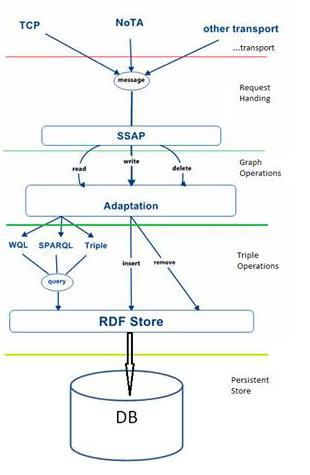
\includegraphics[width=\textwidth]{assets/sib-architecture-2.jpg}
                \caption{Architettura del SIB}
                \label{fig:sib-architecture}
        \end{subfigure}%
        \begin{subfigure}[H]{0.42\textwidth}
                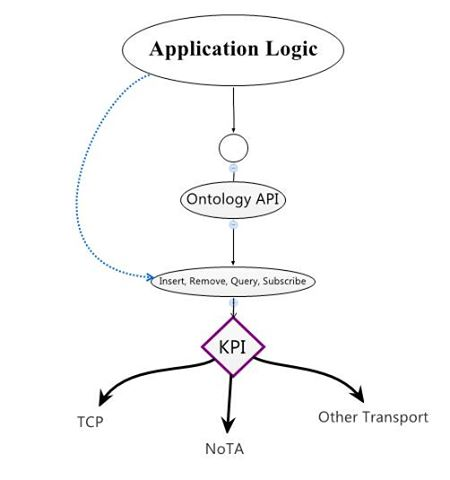
\includegraphics[width=\textwidth]{assets/kp-architecture.jpg}
                \caption{Architettura dei KP}
                \label{fig:kp-architecture}
        \end{subfigure}
        \caption{Architetture SIB e KP}
\end{figure}

\subsection{Le triple RDF}

Nell'architettura Smart-M3 le informazioni sono rappresentate in formato RDF (Resource Description Framework). In RDF le informazioni sono rappresentate in forma di triplette \emph{soggetto, predicato, oggetto}. Le triple vengono memorizzate nel SIB e formano un grafo etichettato diretto che non necessariamente è un grafo connesso.

\subsection{Ontologie}

Mentre RDF fornisce il modello di dati standard per la rappresentazione delle informazioni, l'uso di un linguaggio ontologico è indispensabile per assegnare una semantica all'informazione. Linguaggi ontologici come RDFS e OWL forniscono un vocabolario comune. L'uso di una ontologia comune consente a tutti gli attori (uomini e macchine) di capire reciprocamente la semantica delle informazioni e di cooperare in simbiosi attraverso il SIB. Smart-M3 è agnostico rispetto all'ontologia e quindi consente agli sviluppatori di scegliere il modo migliore di modellare le informazioni per soddisfare le esigenze funzionali del dominio applicativo indirizzato.

\subsection{Sottoscrizioni}

Un aspetto fondamentale di questa tecnologia è il meccanismo delle sottoscrizioni grazie al quale è possibile ricevere notifiche al variare di set di triple. Le sottoscrizioni sono determinanti nella nostra architettura perché, come vedremo più avanti (Sez. ~\ref{sec:protocol}), sono alla base dei protocolli di scambio dati tra i componenti del sistema.

\subsection{SPARQL}

\emph{SPARQL}  (pronuncia sparkle, acronimo ricorsivo di SPARQL Protocol and RDF Query Language) è il linguaggio standard de facto per interrogare dataset RDF. Come si può dedurre dal nome stesso, SPARQL non è semplicemente un linguaggio di interrogazione di dati RDF ma definisce anche il protocollo applicativo utilizzato per comunicare con le sorgenti RDF (si tratta di un binding su HTTP).

Così come SQL riflette nella rappresentazione della query il modello relazionale sottostante, allo stesso modo SPARQL basa la rappresentazione della query sul concetto di tripla e di grafo. Il meccanismo alla base della rappresentazione di una query e della ricerca della sua risposta è il graph matching. La query rappresenta un pattern di un grafo (RDF) e la risposta alla query sono tutte le triple (sotto-grafo) che \emph{fanno match} con il pattern.

\subsection{Il protocollo SSAP}

L'SSAP (\emph{Smart Space Access Protocol}) è il protocollo con cui si comunica con il SIB. Essendo un protocollo session-based, i KP che vogliono comunicare con lo smart-space dovranno prima aderirvi con un operazione di Join prevista dall'SSAP. Il KP fornisce le sue credenziali nel messaggio di Join, il SIB esamina le credenziali e decide se accettare il KP o meno. Dopo l'operazione di Join, il KP può eseguire le altre operazioni. 
L'SSAP è il punto di integrazione principale dell'architettura Smart-M3. Le implementazioni di SIB e KP devono implementare tutte le operazioni del protocollo SSAP per garantire l'interoperabilità.

Le operazioni supportate dal protocollo SSAP sono:

\begin{itemize}
	\item \textbf{JOIN}: Associa il KP allo smart-space solo se le credenziali vengono ritenute valide. Determina l'inizio della sessione.
	\item \textbf{LEAVE}: Determina il termine dell'associazione con lo smart-space e quindi la fine della sessione. Da questo momento in poi non potranno essere eseguite altre operazione di associazione allo smart-space.
	\item \textbf{INSERT}: Operazione atomica di inserzione di un Grafo, formato da triple RDF, nel SIB.
	\item \textbf{REMOVE}: Operazione atomica di rimozione di un Grafo, formato da triple RDF, nel SIB.
	\item \textbf{UPDATE}: Operazione atomica di aggiornamento di un Grafo, formato da triple RDF, nel SIB. In realtà si tratta di una combinazione di DELETE e INSERT eseguita in modo atomico con precedenza dell'operazione di DELETE.
	\item \textbf{QUERY}: Richiesta di informazioni contenute nel SIB attraverso una delle modalità supportate.
	\item \textbf{SUBSCRIBE}: Sottoscrizione a un set di triple contenute nel SIB. Il KP riceve una notifica quando avviene un cambiamento su una di queste triple.
	\item \textbf{UNSUBSCRIBE}: Cancella una sottoscrizione.
\end{itemize}

%\begin{figure}
%	\centering
%	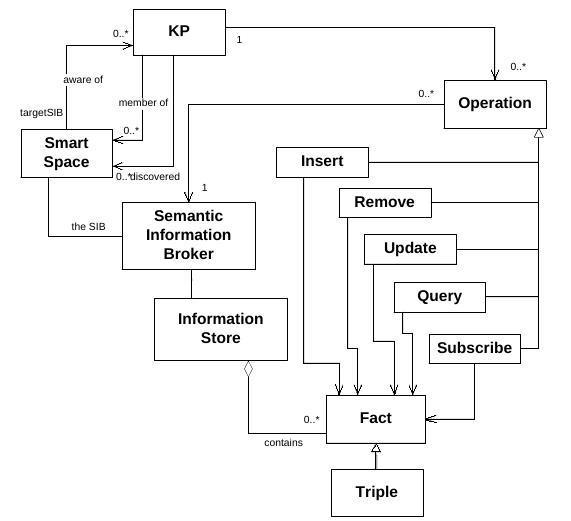
\includegraphics[width=0.5\textwidth]{assets/smart-m3-domain.jpg}
%	\caption{Smart-M3 modello di dominio}
%	\label{fig:smart-m3-domain}
%\end{figure}

\section{Il Modello Ontologico}

In questa sezione cercherò di illustrare come sono stati modellati i dati attraverso una ontologia. Ho ereditato dalla progetto di Tesi di \emph{Federico Montori} (\cite{montori2012}). Io ho contribuito espandendolo per adattarlo ai nuovi requisiti funzionali sorti durante lo sviluppo del progetto. Verranno quindi mostrati gli aspetti dell'ontologia necessari per comprendere il resto della trattazione e verranno approfondite le modifiche da me apportate.

\subsection{Introduzione}

L'ontologia è definibile come una rappresentazione formale ed esplicita di una concettualizzazione condivisa di un dominio di interesse.

L'ontologia presenta le seguenti proprietà:

\begin{itemize}
	\item \textbf{Rappresentazione Formale}: come tale usa un linguaggio logico processabile da elaboratori.
	\item \textbf{Esplicita}: cioè non ambigua e tale da chiarire ogni assunzione fatta.
	\item \textbf{Concettuale}: è una concettualizzazione cioè una vista astratta e semplificata del dominio di interesse.
	\item \textbf{Condivisa}: determinata dal consenso di una pluralità il più ampia possibile di soggetti.
\end{itemize}

Lo scopo delle ontologie è quindi descrivere delle basi di conoscenze, effettuare delle deduzioni su di esse e integrarle tra le varie applicazioni. Per descrivere le ontologie viene utilizzato il linguaggio OWL (\emph{Ontology Web Language}), estensione di RDF. È un linguaggio di markup per rappresentare esplicitamente significato e semantica di termini con vocabolari e relazioni tra gli stessi.

I linguaggi della famiglia OWL sono in grado di creare \emph{classi}, \emph{proprietà}, \emph{istanze} e le relative \emph{operazioni}.


\subsection{Classi di IoE}

Una classe è una collezione di oggetti che corrisponde alla descrizione logica di un concetto. Da una classe si possono creare un numero arbitrario di istanze mentre ad un istanza possono corrispondere una, nessuna o molteplici classi.

Una classe può essere sottoclasse di un'altra classe, ereditando le caratteristiche della super-classe. Tutte le classi sono sottoclasse di \code{owl:Thing}, rappresentazione concettuale di ``cosa''.

Nel modello di dati utilizzato in questo progetto si è cercato di tenere disaccoppiato il concetto di dato dalle altre entità fisiche. Ne consegue che tutte le entità fisiche sono sottoclassi dirette di \code{owl:Thing}, mentre le classi destinate a rappresentare i dati sono sottoclassi di \code{ioe:Data} che a sua volta è sottoclasse di \code{owl:Thing}.

Nel resto di questo documento userò il prefisso \code{ioe:} come abbreviazione di \emph{http://www.m3.com/2012/05/m3/ioe-ontology.owl\#} il namespace scelto per l'ontologia. In generale userò questo prefisso per distinguere le classi dell'ontologia dalle classi Java che come vedremo nella sezione ~\ref{subsec:ioe-lib} hanno lo stesso nome essendo mapping diretto di quest'ultime.

\subsection{Sottoclassi di owl:Thing}\label{subsec:thing}

Come già accennato tutte le entità fisiche del nostro modello ontologico sono sottoclasse diretta di owl:Thing. Quella mostrata di seguito è una lista delle Classi usate in questo progetto omettendo quelle attualmente irrilevanti o inutilizzate.

\begin{description}
	\item \code{ioe:Person}: rappresenta il concetto di persona. Ad ogni persona possono essere associati diversi veicoli (\code{ioe:Vehicle}), diverse richieste di ricarica (\code{ioe:Reservation}) nonché la storia delle ricariche effettuate (\code{ioe:Recharge}). Il concetto di persona viene usato ai fini dell'autenticazione e in un futuro potrà essere determinante ai fini della fatturazione che il provider energetico eseguirà a fronte delle ricariche.
	\item \code{ioe:Vehicle}: rappresenta il concetto di Veicolo Elettrico. Poiché i veicoli NON elettrici sono irrilevanti al fine di questa trattazione è stata usata direttamente questa classe allo scopo. Ad ogni veicolo sono ovviamente associati i dati della batteria (\code{ioe:BatteryData}) che verranno trattati nella sezione relativa alle sottoclassi di \code{ioe:Data} (~\ref{subsec:ioe-data});
	\item \code{ioe:Zone}: Rappresenta l'area di copertura del \emph{City Service}. Essa è definita da un rettangolo formato dall'angolo nord-ovest e dall'angolo sud-est. 
	\item \code{ioe:GridConnectionPoint}: Il \emph{Grid Connection Pointer} (\code{ioe:GCP}) è la stazione di ricarica. Esso contiene almeno un EVSE che invece rappresenta la colonnina dove ci si ricarica effettivamente. Il rapporto tra un GCP e gli EVSE è lo stesso che intercorre tra una stazione di rifornimento e le pompe di benzina. 
	\item \code{ioe:EVSE}: Il \emph{Electrical Vehicle Supply Equipment} è il punto in cui il veicolo si connette alla rete elettrica. Una volta connesso può sia ricaricare la sua batteria che cedere energia alla smart-grid. Un EVSE ha diversi connettori (\code{ioe:Connector}) per adattarsi ai vari tipi di presa posseduti dai veicoli elettrici. Inoltre, ogni EVSE, ha una lista di prenotazioni associate.
	\item \code{ioe:ChargeProfile}: È l'insieme dei parametri che caratterizzano il profilo energetico di un EVSE in un determinato istante. I parametri attualmente sono: potenza, orario di validità del profilo stesso e prezzo per unità di energia (in genere 1 kWh). Ovviamente può essere attivo un solo \code{ioe:ChargeProfile} alla volta e il variare di quest'ultimi può essere determinato da fasce orarie proprio come avviene per l'energia elettrica casalinga.
	\item \code{ioe:Connector}: È il connettore di ricarica ovvero il punto i contatto tra l'EVSE e l'EV. Ogni EVSE può avere diversi connettori al fine di poter essere compatibile con il maggior numero di veicoli possibile. Malgrado negli usa si stia cercando di introdurre uno standard a riguardo ormai esistono diversi tipi di connettori. 
	\item \code{ioe:ChargeRequest}: Richiesta di ricarica. Viene istanziata quando un utente necessita di creare una prenotazione e al suo interno sono contenuti tutti i parametri necessari a descriverla. Fa parte del protocollo di richiesta di prenotazione discusso nella sezione ~\ref{sec:protocol}. Mentre un approfondimento sulla sua struttura è trattato nella sezione ~\ref{subsubsec:chargerequest}.
	\item \code{ioe:ChargeResponse}: È la risposta fornita dal servizio cittadino a seguito della richiesta di prenotazione. Al suo interno contiene un riferimento alla richiesta (\code{ioe:ChargeRequest}) da cui è stata generata e una lista di opzioni di ricarica che aderiscono alla richiesta dell'utente (\code{ioe:ChargeOption}).
	\item \code{ioe:ChargeOption}: Fa parte della risposta(\code{ioe:ChargeResponse}) che il servizio cittadino da all'utente in seguito a una richiesta di prenotazione (\code{ioe:ChargeRequest}). Contiene i parametri di ricarica come EVSE, orario e prezzo. 
	\item \code{ioe:Currency}: Rappresenta una valuta relativa a un prezzo. Alcune sue istanze sono state inserte direttamente nell'ontologia (\code{ioe:Euro}, \code{ioe:Dollar} ecc..);
	\item \code{ioe:Reservation}: Se il protocollo di richiesta di prenotazione va a buon fine verrà creata un istanza di questa classe che indica che l'EVSE a cui è associata è occupato per un determinato periodo di tempo. 
	\item \code{ioe:ReservationList}: Lista di prenotazioni associate ad un EVSE. Ogni EVSE può avere un unica lista di prenotazioni associata.
	\item \code{ioe:ReservationRetire}: Classe che denota la volontà dell'utente di ritirare una prenotazione.
	\item \code{ioe:Recharge}: Quando un utente, in seguito a una prenotazione, termina di ricaricarsi, inserita questa entità ad esso associato. Denota l'avvenuta ricarica è può essere utile per tener traccia dell'attività dell'utente nonché per fare statistiche.
	\item \code{ioe:UnityOfMeasure}: Rappresenta l'unità di misura per i dati del progetto. Deve esserne associata una ad ogni sottoclasse di \code{ioe:Data}. Attualmente sono hardcoded all'interno dell'ontologia (\code{ioe:Watt}, \code{ioe:Volt} ecc..) 	
	\item \code{ioe:Data}: Questa classe rappresenta il concetto di dato misurabile e ogni sua sottoclasse sarà caratterizzata da un valore e da un unità di misura.
\end{description}

\subsection{Sottoclassi di ioe:Data}\label{subsec:ioe-data}

In questa sezione viene mostrata una lista di tutte le tipologie di dato utilizzate in questo progetto. Esse sono tutte sottoclassi di \code{ioe:Data} e sono caratterizzate da un valore e da unità di misura \code{ioe:UnityOfMeasure}. Le unità di misure che vengono elencate nel seguente elenco sono quelle utilizzate nell'ambito di questo progetto niente vieta di cambiarle.

\begin{description}
	\item \textbf{BatteryData}: In questa classe sono raggruppati tutti i dati relativi allo stato della batteria di un veicolo (ChargeData, VoltageData, PowerData, CurrentData, TempertureData)
	\item \textbf{ChargeData}: Rappresenta la quantità di carica, l'unità di misurata usata è il kilowattora (kWh).
	\item \textbf{VoltageData}: Rappresenta la tensione elettrica, l'unità di misurata usata è il volt (V).
	\item \textbf{PowerData}: Rappresenta la potenza elettrica, l'unità di misurata usata è il kilowatt (kW). 
	\item \textbf{CurrentData}: Rappresenta l'intensità di corrente, l'unità di misurata usata è l'ampere (A). Usato sia per indicare la corrente in uscita che quella in entrata, come ad esempio i cicli di carica e scarica della batteria.
	\item \textbf{TempertureData}: Rappresenta la temperatura, l'unità di misurata usata è il grado celsius (\textcelsius). Attualmente non è considerato nei nostri modelli.
	\item \textbf{LocationData}: Rappresenta i dati geografici dell'entità a cui si riferisce. In realtà non viene mai utilizzato ma viene usata direttamente la sua sottoclasse GPSData.
	\item \textbf{GPSData}: Rappresenta le coordinate GPS ovvero latitudine e longitudine, l'unità di misura non 
	\item \textbf{SpatialRangeData}: Rappresenta uno spazio geografico determinato da un punto GPS e un raggio intorno ad esso, l'unità di misurata usata è il metro (m).
	\item \textbf{PriceData}: Rappresenta le informazioni relative a un prezzo ad esso è associata una valuta (sezione ~\ref{subsec:thing})
	\item \textbf{TimeIntervalData}: Rappresenta un intervallo di tempo compreso tra due date. Originariamente veniva usato con le date nella forma gg/mm/aa, attualmente invece vengono indicati gli intervalli in millisecondi.
\end{description}

\subsection{Modifiche apportate all'ontologia}

La versione dell'ontologia su cui ho iniziato a lavorare era la \emph{1.5.4} dalla quale sono seguiti 10 successivi rilasci fino ad arrivare alla versione attuale \emph{1.6.2}. Le modifiche più importanti sono state quelle relative al supporto di un nuovo protocollo di prenotazione delle ricariche, inoltre sono state operate operazioni di refactoring e di correzione di errori.

\subsubsection{Il concetto di Utente}\label{subsubsec:person}

Inizialmente il concetto di utente non era previsto nell'ontologia in quanto non trovava nessuna applicazione pratica.
L'entità che interagiva con la smart-grid era il veicolo e non l'utente. Questo approccio presenta i suoi limiti nel caso in cui un utente possieda più veicoli e voglia monitorare le ricariche effettuate o le prenotazioni pendenti con un unica soluzione. Inoltre, anche dal punto di vista dei fornitori di corrente elettrica, può essere utile avere una visione a livello di utente in modo da semplificare le operazioni di fatturazione. 
Successivamente è stata introdotta la necessità di autenticare gli utenti al fine di poter cifrare le comunicazioni con l SIB. 

È stata quindi introdotta la classe \code{ioe:Person}. Seppur esistano già delle ontologie con delle classi che rappresentano questo concetto è stato ritenuto più semplice crearne uno nostro. Sviluppi futiri potrebbero legare questo concetto a uno già esistente in modo da rendere più semplice l'interoperabilità tra sistemi diversi. La classe presenta le seguenti proprietà:

\begin{itemize}
	\item \code{ioe:hasName}: Nome e cognome dell'utente in formato stringa. Attualmente è irrilevante avere una separazione dei due. 
	\item \code{ioe:hasUserIdentifier}: Codice che identifica univocamente l'utente.
	\item \code{ioe:hasVehicle}: Questa proprietà associa a un utente uno o più veicoli.
\end{itemize}

\noindent
Come si può vedere attualmente l'utente è modellato in modo molto primitivo, sono state infatti incluse solo le proprietà strettamente necessarie al nostro dominio di interesse. 

\subsubsection{Il concetto di Veicolo}\label{subsubsec:vehicle}

Nel vecchio modello ontologico il concetto di veicolo, in quanto non essenziale, non veniva particolarmente enfatizzato. Nella ultime versioni dell'ontologia ho aggiunto alcune proprietà al veicolo per venire incontro all'esigenza di poter distinguere la provenienza dei veicoli stessi. Infatti i veicoli vengono inseriti nel SIB dal simulatore e possono anche essere reali come nel caso del Fiat Daily provato al CRF (App. ~\ref{app:crf}).

Il veicolo è attualmente definito dalle seguenti proprietà:

\begin{itemize}
	\item \code{ioe:hasManufacturer}: Casa automobilistica che produce il veicolo.
	\item \code{ioe:hasModel}: Modello del veicolo.
	\item \code{ioe:hasGPSData}: Questa proprietà punta ad un istanza di \code{ioe:GPSData} che a sua volta contiene le informazioni di latitudine e longitudine.
	\item \code{ioe:hasBatteryData}: Questa proprietà punta ad un istanza di \code{ioe:BatteryData} che contiene tutti i dati della batteria.
	\item \code{ioe:hasIdentificationData}: Identificativo del veicolo, attualmente non viene usato e per semplificazione al suo posto viene usata la proprietà \code{ioe:hasName}.
\end{itemize}

Precedentemente 


\subsubsection{Il concetto di Ricarica}

Nella prime versioni dell'ontologia non esisteva nulla che indicasse il concetto di "ricarica avvenuta" molto utile al fine di far statistiche sia lato utente (es: quanto si è speso in un mese per ricaricare il veicolo) sia lato smart-grid (es: Quanta energia è stata erogata, quali sono stati gli introiti). Questo perché i tempi previsti dalla prenotazione possono differire sensibilmente da quelli reali, basti pensare a una persona che arriva in ritardo a ricaricarsi o lascia la colonnina in anticipo. 

%\paragraph{Coordinamento con AICIA} È stato inoltre necessario dimostrare l'interoperabilità con un altro partner di IoE ovvero AICIA. Questo al fine di dimostrare il buon lavoro di partnership tra i membri di IoE 

È stata quindi introdotta la classe \code{ioe:Recharge}, da notare che le proprietà di seguito elencate sono state accordate con un altro partner del progetto IoE ovvero la spagnola AICIA al fine di eseguire un demo congiunta dove si dimostrava l'interoperabilità tra la nostra piattaforma e quella sviluppata da loro.

\begin{itemize}
	\item \code{ioe:hasDate}: Data e ora in cui è avvenuta la ricarica.
	\item \code{ioe:hasUser}: Utente che ha effettuato la ricarica, qui si nota la necessità di inserire la classe \code{ioe:Person} (~\ref{subsubsec:person}).
	\item \code{ioe:hasRechargeTime}: Il tempo necessario ad eseguire la ricarica.
	\item \code{ioe:hasConsumption}: La quantità di corrente impiegata per effettuare la ricarica.
\end{itemize}

\subsubsection{Il Vecchio Protocollo di Prenotazione}\label{subsubsec:old-proto}

Il protocollo di prenotazione iniziale era in stato embrionale e serviva a scopo esemplificativo per dimostrare la fattibilità della cosa. I parametri previsti per la richiesta di richiesta, ovvero come proprietà della classe \code{ioe:ChargeRequest} erano:

\begin{itemize}
	\item \code{ioe:hasPreferredTime}: Indica la data in cui l'utente vorrebbe effettuare la ricarica.
	\item \code{ioe:hasPosition}: Indica la posizione da cui si sta eseguendo la richiesta.
	\item \code{ioe:hasRequestedEnergy}: Indica la quantità di carica richiesta. 
	\item \code{ioe:hasRequestingVehicle}: Indica il veicolo che richiede la ricarica.
	\item \code{ioe:hasChargeResponse}: Indica la risposta che viene fornita dal sistema.
\end{itemize}

\noindent
In quanto embrionale in seguito ad alcune simulazioni è sorta la necessità di aggiornare il protocollo per risolvere alcune problematiche. \\ 
Al di la della mancanza del concetto di utente, l'assenza di range nei campi \code{ioe:hasPreferredTime} ed \code{ioe:hasPosition} potevano portare ad ambiguità nella risposta che non avendo alcun limite poteva diventare eccessivamente grande. Questo poteva portare problemi di traffico nel caso di utilizzo di smartphone agganciati alla rete tramite connettività mobile.

\subsubsection{Il nuovo Protocollo di prenotazione}\label{subsubsec:chargerequest}

In seguito ai problemi messi in luce nel paragrafo precedente (~\ref{subsubsec:old-proto}) è stato deciso di sviluppare un nuovo protocollo di prenotazione che prendesse in considerazioni i nuovi requisiti funzionali.

La classe è \code{ioe:ChargeRequest} è stata quindi ridefinita con le seguenti proprietà:

\begin{itemize}
	\item \code{ioe:hasRequestingUser}: Utente che ha effettuato la ricarica. Malgrado si possa risalire all'utente tramite il veicolo è stato comunque inserita la proprietà al fine di semplificare le query SPARQL.
	\item \code{ioe:hasSpatialRange}: Area nella quale si vuole eseguire la ricarica. Il punto centrale di quest'area non corrisponde necessariamente con la posizione dell'utente. Come vedremo nella sezione relativa all'applicazione mobile (~\ref{chap:mobile-app}) l'area di prenotazione può essere scelta arbitrariamente sulla mappa.
	\item \code{ioe:hasTimeInterval}: Indica il range temporale all'interno del quale si è disposti ad eseguire la ricarica. Può anche essere molto superiore al tempo necessario per la ricarica nel caso in cui non ci siano particolari preferenze di tempo.
	\item \code{ioe:hasRequestingVehicle}: Indica il veicolo per cui si richiede la ricarica. Non differisce rispetto al vecchio protocollo.
	\item \code{ioe:hasRequestedEnergy}: Indica la quantità di carica richiesta. Non differisce rispetto al vecchio protocollo.
\end{itemize}

\noindent
Per quanto sia stato migliorato il protocollo è ancora incompleto ed in quanto tale è ancora aperto a migliorie. Ad esempio non è possibile specificare la volontà dell'utente di essere più flessibile per quanto riguarda la quantità di carica richiesta e nemmeno, nel caso fosse richiesto dalla smart-grid, se fosse disposto a cedere parte della sua carica.
\\ \\
Oltre alla richiesta è stata modificata anche la risposta. Alla classe \code{ioe:ChargeResponse} è stata aggiunta la proprietà \code{ioe:hasRelatedRequest} al fine di semplificare le query SPARQL.
Anche le opzioni di ricarica contenute nella risposta sono state modificate con lo scopo di farle aderire ai nuovi requisiti funzionali ma anche per semplificare le query SPARQL.

Di seguito verranno esposte le proprietà della classe \code{ioe:ChargeOption}. Dalla vecchia definizione è stata rimossa la proprietà \code{ioe:hasChargeProfile}. Le proprietà ereditate dalla vecchia ontologia verranno opportunamente segnalate.

\begin{itemize}
	\item \code{ioe:optionHasEVSE}: EVSE presso il quale avverrà la ricarica (ereditata).
	\item \code{ioe:hasTimeInterval}: Specifica il tempo necessario a ricaricarsi calcolato sulla base dell'energia richiesta e la potenza della colonnina. Questa proprietà era presente anche nella vecchia definizione dove i tempi venivano indicati con le date in formato gg/mm/aaaa, attualmente i tempi vengono indicati in millisecondi (passati dalla mezzanotte del 1 Gennaio 1970 UTC) con le proprietà \code{ioe:hasFromTimeMillisec} e \code{ioe:hasToTimeMillisec}.
	\item \code{ioe:hasRequestingVehicle}: Il veicolo per cui è stata effettuata la richiesta. (ereditata)
	\item \code{ioe:hasRequestingUser}: L'utente che ha effettuato la richiesta.
	\item \code{ioe:hasGridConnectionPoint}: Il GCP presso cui avverrà la ricarica. Malgrado vi si possa accedere tramite l'EVSE è stato inserito al fine di semplificare le query SPARQL.
	\item \code{ioe:hasTotalPrice}: Prezzo totale della ricarica.
	\item \code{ioe:hasGcpPosition}: Posizione del GCP, anche questa proprietà è stata aggiunta per semplificare le query SPARQL.
\end{itemize}


\subsubsection{Rimozione informazioni Hardcoded}

Fino alla versione \emph{1.5.11} dell'ontologia le informazioni relative ai GCP erano hardcoded nell'ontologia, scelta che all'inizio del progetto è stata necessaria a causa del poco tempo. Successivamente questo approccio ha si è rivelato fortemente limitante in quanto la modifica dell'ontologia è un operazione abbastanza tediosa e sopratutto è poco flessibile. 

Al fine di risolvere questo problema ho deciso di rimuovere questi dati dall'ontologia e inserirli all'interno di un file XML che viene caricato dal \emph{City Service} (Sez. ~\ref{subsubsec:city-init}) e dal simulatore (Sez. ~\ref{chap:sim}) in fase di inizializzazione.

Grazie a questo approccio è diventato relativamente semplice impostare uno scenario del tutto diverso da quello previsto dal progetto.

\section{I Semantic Information Broker}

I SIB sono alla base dell'infrastruttura semantica che caratterizza questo progetto. I componenti del sistema (dal servizio cittadino, allo smartphone, all'EVSE ecc..) comunicano e rendono permanenti le informazioni grazie ad essi. L'architettura rimane sostanzialmente invariata da quella presentata da Federico Montori (\cite{montori2012}) nel suo progetto di tesi. Verrà comunque esposta al fine di comprendere il resto della trattazione e verranno evidenziate le variazioni apportate alla soluzione iniziale.

L'architettura proposta prevede 2 SIB: il \emph{City SIB} e il \emph{Dash SIB}.

\subsection{City SIB}\label{subsec:city-sib}

Il \emph{City SIB} è il SIB cittadino. Al suo interno vengono immagazzinate tutte le informazioni utili a caratterizzare uno scenario di mobilità elettrica veicolare. Viene inoltre utilizzato come interfaccia di scambio dati tra il \emph{City Service} e gli agenti esterni, infatti è qui che vengono scritti i messaggi che compongono i protocolli i quali vengono cancellati una volta terminati. L'area di copertura di tale SIB e di conseguenza del \emph{City Service} è definita dalla classe dell'ontologia \code{ioe:Zone} anche se attualmente non viene utilizzata in quanto gli scenari proposti prendono in considerazione una città alla volta.

Al fine di poter rispondere alle richieste di prenotazione degli utenti il \emph{City Service} contiene le informazioni su tutte le colonnine della zona che ricopre. Inoltre possiede le informazioni relative agli utenti e a i veicoli da essi posseduti. Non contiene le informazioni relative alla batteria che sono contenute nella \emph{Dash SIB} (~\ref{subsec:dash-sib}). Nell'architettura proposta nel progetto precedente a questo gli utenti non esistevano (~\ref{subsubsec:person}) e le informazioni relative ai veicoli si trovavano esclusivamente nella \emph{Dash SIB}.

L'inizializzazione del \emph{City SIB}, contrariamente a quanto avveniva prima, viene eseguita dal servizio cittadino stesso, inoltre il servizio cittadino si occupa di caricare le informazioni dei GCP, caricate da un file XML, e di inserirle nel SIB (Sez. ~\ref{subsubsec:city-init}).


\subsection{Dash SIB}\label{subsec:dash-sib}

Il \emph{Dash SIB} è  un SIB che dovrebbe essere integrato a bordo di ogni veicolo. Il suo scopo è tenere costantemente traccia dei parametri che caratterizzano posizione, stato della batteria e tutti gli altri parametri variabili che caratterizzano un veicolo. Al fine di collegare questi dati a un veicolo la tripla che descrive un istanza di \code{ioe:Vehicle} viene ripetuta anche su questa SIB. 

Inizialmente si pensava che questo SIB sarebbe stato eliminato in un contesto reale in quanto i dati in esso contenuti sarebbero stati presi direttamente dal veicolo. È stato invece deciso di mantenerlo per poterlo usare come interfaccia comune per l'interrogazione dei dati. Ovvero le applicazioni che utilizzano i dati del veicolo, come ad esempio l'applicazione mobile, dovrebbero essere agnostiche dalla sorgente di dati (es: Veicolo Reale, Veicolo Simulato). Compito del programmatore è scrivere un adattatore che scrive i dati in provenienti dalle varie fonti sul \textsc{Dash SIB}. Come vedremo più avanti (Cap. ~\ref{chap:sim}, ~\ref{chap:mobile-app}) grazie a questa tecnica è possibile controllare dal telefonino un veicolo presente nel simulatore tenendone monitorati tutti i parametri. I veicoli del simulatore scrivono tutti sullo stesso \emph{Dash SIB} in quanto sarebbe computazionalmente proibitivo e del tutto inutile fare altrimenti.

Siccome attualmente non esistono veicoli che contengono un SIB esiste in fase di test su veicolo reale (App. ~\ref{app:crf}) è stato necessario portare un computer a bordo che contenesse il \textsc{Dash SIB} dal quale l'applicazione mobile attingeva per prelevare i dati.

\section{La libreria IoE}\label{subsec:ioe-lib}

Questa libreria implementa la logica applicativa ovvero il nucleo operativo del nostro strato di servizi. È la base per qualunque applicazione che intenda in interfacciarsi con il sistema in modo semplice ed efficace. Viene infatti sfruttata sia dal \emph{City Service} che dall'applicazione mobile, da me sviluppati, è inoltre utilizzata da un visualizzatore di ricariche, nato da un progetto parallelo al mio, del quale sviluppo si è occupata una ragazza di Ingegneria.

\subsection{Connessione al SIB}

La connessione al \emph{SIB} viene eseguita da una libreria Java (JavaKPI), sviluppata da ARCES, che implementa il protocollo SSAP. Ho creato un wrapper di questa libreria che ne semplifica l'utilizzo e aggiunge alcune funzionalità. Essa si trova nel package \code{it.unibo.ioe.sib}.

\subsubsection{RdfTriple}
La libreria JavaKPI rappresenta le triple RDF come vettore di Stringhe di 5 elementi (\code{Vector<String>}): soggetto, predicato, oggetto, tipo soggetto, tipo oggetto. 
Per semplificare la gestione delle triple RDF, che sono l'entità di base su cui si basa il SIB, ho creato una classe \code{RdfTriple} che possiede gli attributi \code{subject},\code{predicate}, \code{object}, \code{subjectType}, \code{objectType} e i corrispettivi \code{getter} e \code{setter}.


\subsubsection{KpConnector}

La maggior parte delle operazioni che si possono eseguire con la libreria JavaKPI richiedono due passaggi: l'invio del comando, e il parsing della risposta. Questo perché ogni operazione di interazione con il SIB avviene tramite messaggi XML, conformi al protocollo SSAP. La libreria genera automaticamente il messaggio da inviare alla SIB ma lascia al programmatore l'onere di effettuare il parsing della risposta. Ho quindi mappato tutte le operazioni di interazione con la SIB all'interno della classe \code{KpConnector}.

La classe \code{KpConnector} svolge le operazioni di parsing anche sui messaggi di risposta. Al posto dei vettori di stringhe ho utilizzato istanze della classe \code{RdfTriple}. Mentre dove venivano usate liste di triple (es: inserimento multiplo di triple, risultati di query SPARQL) ho sostituito con liste di oggeti di tipo \code{RdfTriple} (\code{List<RdfTriple>}). La classe che si occupa di convertire i tipi di dato usati dalla libreria \code{JavaKPI} ai tipi usati dal wrapper da me creato è \code{RdfParser}.

\subsubsection{KpFactory}

La classe \code{KpConnector} necessita di indirizzo, porta e nome del SIB a cui ci si vuole connettere, questo perché il suo utilizzo deve essere il più generico possibile. Nel nostro caso però le connessioni avvengono sempre verso gli stessi due SIB (CITY e DASH), ho quindi creato una classe factory (\code{KpFactory}) che, conoscendo i parametri di connessione necessari, crea due istanze di \code{KpConnector}, una per il CITY SIB e una per il DASH SIB, e restituisce sempre quello evitando quindi la creazione di istanze di oggetti inutili. Essendo la libreria \code{JavaKPI} non thread-safe viene comunque data la possibilità di creare istanze in modo veloce nel caso si lavori in ambienti multi-thread. Questo aspetto verrà approfondito più avanti dove vedremo come, tramite la tecnica dei pool di oggetti, possiamo risparmiare il tempo necessario a creare nuove istanze.

%http://sourceforge.net/projects/smartm3-javakpi/

\subsection{Entities}

Ogni classe dell'ontologia è stata mappata con una rispettiva classe Java (Entity) nel package \code{it.unibo.ioe.entity} . Per questa scelta architetturale mi sono ispirato all'ORM (Object Relational Mapping) che è una tecnica di programmazione che favorisce l'integrazione di sistemi software aderenti al paradigma della programmazione orientata agli oggetti con sistemi RDBMS (Relational database management system). %http://it.wikipedia.org/wiki/Object-relational_mapping

\subsubsection{Mapping} 

Il mapping che ho creato è molto semplice e tiene conto solo delle proprietà strettamente necessarie nello strato di servizi e tralascia alcuni dettagli come l'unità di misura che attualmente, malgrado siano previsti nell'ontologia, vengono dati per scontati a livello applicativo.
Le proprietà delle classi che hanno come oggetto un letterale sono state mappate con tipi primitivi Java (\code{int},\code{double},\code{String} ecc..). Mentre le proprietà che come oggetto hanno un'altra classe sono rappresentate come attributo che come tipo ha l'Entity
che corrisponde alla classe. 

\subsubsection{Serializzazone} 

Alcune Entity sono state opportunamente annotate al fine di poter essere serializzate in XML tramite la tecnologia \code{JAXB}. Questo è risultato necessario nel caso dei \emph{GCP} che vengono caricati da un file XML, nella cartella del \emph{City Service}, il quale si occupa poi di inserirli nel SIB. Ogni classe inoltre implementa l'interfaccia \code{java.io.Serializable} al fine di permettere il passaggio delle Entity tra le varie \code{Activity} dell'applicazione mobile.

\paragraph{Esempio}

La proprietà dell'ontologia \code{ioe:hasEVSE} ha come dominio \\ \code{ioe:GridConnectionPoint} e come codominio \code{ioe:EVSE}. Inoltre tutte le classi dell'ontologia hanno al proprietà code{vcard:hasName}.

Questa situazione viene tradotta nell'Entity:

\begin{java}[caption={Entity di esempio},label=lst:entity]
@XmlRootElement(name = "GCP")
@XmlAccessorType(XmlAccessType.FIELD)
public class GCP implements Serializable {
	@XmlTransient
	private String URI;
	private String gcpName;
	@XmlElement(name = "EVSE")
	private List<EVSE> evseList;
	/* other properties*/
	/* getter & setter*/	
}
\end{java}

\subsection{Controller}

I \code{Controller} sono le classi delegate ad eseguire le operazioni \code{CRUD} (create, read, delete, update) con il SIB e si trovano nel package \code{it.unibo.ioe.controller}. Ne esiste uno per ogni Entity. Ogni \code{Controller} possiede un istanza di \code{KpConnector} che permette la comunicazione con il SIB. 

\begin{description}
	\item \textbf{Lettura} Le operazioni di lettura vengono eseguite tramite una query \code{SPARQL} che preleva dal SIB le informazioni necessarie che poi vengono inserite in una nuova istanza di Entity la quale viene restituita all'utente.

	\item \textbf{Scrittura} Le operazioni di scrittura ricavano una lista di triple RDF a partire da un istanza di Entity. La lista di triple viene poi convertita in una \code{SPARQL} insert al fine di ridurre i dati inviati al SIB. L'operazione di conversione è eseguita da una funzione di della  classe \code{SibUtil}. Questa tecnica si rivela particolarmente utile quando si utilizza la libreria da un dispositivo mobile connesso a internet tramite rete cellulare (es: EDGE, GPRS, HSDPA ecc\dots). Da notare che tutte le Entity possiedono un campo \code{URI} che viene valorizzato nell'operazione di inserzione con l'URI assegnato all'istanza che si sta per scrivere sul SIB. 

	\item \textbf{Aggiornamento} Le operazioni di aggiornamento ricavano i dati aggiornati tramite una query \code{SPARQL} che andranno a sostituire quelli obsoleti all'intenro di un istanza di Entity

	\item \textbf{Rimozione} Le operazioni di rimozione lato \emph{City Service} sono eseguite direttamente tramite \code{SPARQL} delete. Mentre le operazioni di rimozione all'esterno (es. applicazione mobile), per motivi di sicurezza, sono eseguite tramite richiesta al servizio cittadino il quale si occupa di effettuare la rimozione vera e propria.
\end{description}













